\documentclass[11pt,a4paper]{article}
\usepackage[T1]{fontenc}
\usepackage[utf8]{inputenc}
\usepackage{lmodern}
\usepackage{amsmath,amssymb,amsthm,mathtools,mathrsfs}
\usepackage{graphicx,float,xcolor,multicol}
\usepackage[shortlabels]{enumitem}
\usepackage[margin=27mm]{geometry}
\usepackage{microtype,needspace,placeins}
\usepackage{tikz,tikz-cd}
\usetikzlibrary{arrows.meta,calc,positioning,patterns,decorations.pathreplacing}
\usepackage[colorlinks=true,linkcolor=teal,urlcolor=teal,citecolor=teal]{hyperref}
\setlength{\parindent}{0pt}
\setlength{\parskip}{.6em}
\setcounter{secnumdepth}{0}
\allowdisplaybreaks
\raggedbottom
\providecommand{\cross}{\times}
\DeclareUnicodeCharacter{2020}{\ensuremath{\dagger}}
\DeclareMathOperator{\supp}{supp}
\DeclareMathOperator*{\esssup}{ess\,sup}
\providecommand{\chapter}{\section}
\newenvironment{tool}[2]{\subsection*{Tool #1 --- #2}}{}
\newcommand{\ToolRef}[1]{Tool #1}
\newcommand{\FigureTag}[2]{\textit{Figure #1}}
\newcommand{\Result}[1]{\subsection*{#1}}
\newcommand{\Application}[1]{\subsubsection*{Application\if\relax\detokenize{#1}\relax\else\space--- #1\fi}}
\newcommand{\ProofHeading}{\par\textit{Proof.}\space}
\newcommand{\ProofOf}[1]{\par\textit{Proof of #1.}\space}
\newcommand{\RemarkHeading}{\par\textbf{Remark.}\space}
\newcommand{\NoteHeading}{\par\textbf{Note.}\space}
\newcommand{\ExerciseHeading}{\par\textbf{Exercise.}\space}

% Rendering support only; mathematical text is in each independent post.
\usepackage{booktabs,array,longtable}
\definecolor{HandoutBlue}{HTML}{2F6690}
\definecolor{HandoutNavy}{HTML}{17365D}
\newtheorem{theorem}{Theorem}
\newtheorem{lemma}[theorem]{Lemma}
\newtheorem{proposition}[theorem]{Proposition}
\newtheorem{corollary}[theorem]{Corollary}
\newtheorem{conjecture}[theorem]{Conjecture}
\newtheorem{definition}{Definition}
\newtheorem{example}{Example}
\newtheorem{namedtoolcounter}{Tool}
\newenvironment{namedtool}[1]{\begin{namedtoolcounter}[#1]}{\end{namedtoolcounter}}
\newtheorem*{claim}{Claim}
\newtheorem*{remark}{Remark}
\newtheorem*{exercise}{Exercise}
\newtheorem*{question}{Question}
\newtheorem*{observation}{Observation}
\newcommand{\SourceChapter}[2]{\section*{#2}}
\newcommand{\Lecture}[2]{\section*{Lecture #1: #2}}
\newcommand{\unclear}[1]{\textit{[unclear: #1]}}
\newcommand{\sourcegap}{\textit{[unfinished in the source]}}
\DeclareMathOperator{\dist}{dist}
\DeclareMathOperator{\id}{id}
\DeclareMathOperator{\Hol}{Hol}
\DeclareMathOperator{\Per}{Per}
\DeclareMathOperator{\Fix}{Fix}
\DeclareMathOperator{\diam}{diam}
\DeclareMathOperator{\Var}{Var}
\DeclareMathOperator{\Leb}{Leb}
\DeclareMathOperator{\Hom}{Hom}
\DeclareMathOperator{\End}{End}
\DeclareMathOperator{\Ann}{Ann}
\DeclareMathOperator{\Spec}{Spec}
\DeclareMathOperator{\Max}{Max}
\DeclareMathOperator{\Ob}{Ob}
\DeclareMathOperator{\Tor}{Tor}
\DeclareMathOperator{\Ass}{Ass}
\DeclareMathOperator{\Mor}{Mor}
\DeclareMathOperator{\Fun}{Fun}
\DeclareMathOperator{\Nat}{Nat}
\DeclareMathOperator{\Cone}{Cone}
\DeclareMathOperator{\MCG}{MCG}
\DeclareMathOperator{\Aut}{Aut}
\DeclareMathOperator{\Deck}{Deck}
\DeclareMathOperator{\SL}{SL}
\DeclareMathOperator{\PSL}{PSL}
\DeclareMathOperator{\Area}{Area}
\DeclareMathOperator{\im}{im}
\DeclareMathOperator{\PSh}{PSh}
\newcommand{\CRing}{\mathsf{CRings}}
\newcommand{\AMod}{A\text{-}\mathsf{Mod}}
\newcommand{\Ab}{\mathsf{Ab}}
\newcommand{\Z}{\mathbb Z}
\newcommand{\Q}{\mathbb Q}
\newcommand{\R}{\mathbb R}
\newcommand{\C}{\mathbb C}
\newcommand{\N}{\mathbb N}
\newcommand{\kk}{\mathbb k}
\renewcommand{\aa}{\mathfrak a}
\newcommand{\bb}{\mathfrak b}
\newcommand{\pp}{\mathfrak p}
\newcommand{\qq}{\mathfrak q}
\newcommand{\mm}{\mathfrak m}
\newcommand{\nn}{\mathfrak n}
\newcommand{\rad}{\mathrm r}
\newcommand{\cat}[1]{\mathsf{#1}}
\setcounter{secnumdepth}{0}
\allowdisplaybreaks

\graphicspath{{figures/complex-dynamics-notes/}}
\begin{document}
\section*{Parabolic Fixed Points and the Flower Theorem}
% BLOG-CONTENT-BEGIN
Consider a fixed point $f(\widehat p)=\widehat p$ whose multiplier satisfies $\lambda^q=1$ and for which $f^{\circ q}$ is not locally the identity. Such points are called parabolic fixed points. It is immediately clear that the expected dynamics should be different. For instance, consider the orbits of $\pm1$ and $\pm i$ under $f(z)=z+z^3$.
\begin{figure}[H]\centering
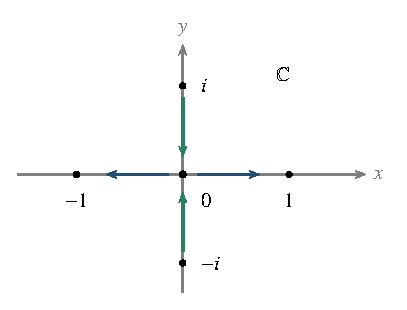
\includegraphics[width=.55\textwidth]{cd3-fig-01.pdf}
\FigureTag{CD3.1}{fig:cd3-01}
\end{figure}
The map $f$ repels $1,-1$ and attracts $i,-i$ towards $\widehat p=0$. Notice that it pushes and pulls from two directions. The following theorem tells us that such patterns reappear. For now, no neighbourhood of $\widehat p=0$ can be expected to be a ``basin'', since $\widehat p$ is a sink only in certain directions.
% Source page 2
\setcounter{definition}{10}\begin{definition}
Let $f(z)=z+az^{n+1}+O(z^{n+2})$. A vector $v\in\mathbb C$ is attracting if $nav^n=-1$, and repelling if $nav^n=+1$.
\end{definition}
\begin{remark}
The equation $nav^n=\pm1$ has $2n$ equally spaced solutions. Also $f$ is locally invertible, with $f^{(n+1)}(0)\ne0$, $f'(0)=1$, and $f^{(k)}(0)=0$ for $1<k\le n$. Thus
\[
(f^{-1})''(0)=-\frac{f''(0)}{(f'(0))^3}=-2a\quad(n=1),
\]
and
\[
(f^{-1})'''(0)=\frac{3(f''(0))^2-f'(0)f'''(0)}{(f'(0))^5}
=-f'''(0)=-6a\quad(n=2).
\]
Inductively, $-f^{(n+1)}(0)=(f^{-1})^{(n+1)}(0)$. Thus attracting and repelling vectors exchange roles for $f^{-1}$.
\end{remark}
The next theorem explains why these vectors have their names, and shows that all maps with a parabolic point behave somewhat like $z+z^3$.
\setcounter{theorem}{16}\begin{theorem}\label{cd3:asymptotic}
If an orbit $\{z_k\}_k$ of $z_0$ tends to $0$ and $z_k\ne0$ for every $k$, then $z_k\sim v_j/k^{1/n}$ as $k\to\infty$ for some attracting vector $v_j$. The analogous assertion holds for orbits converging to $0$ under $f^{-1}$.
\end{theorem}
% Source page 3
\begin{proof}
We conjugate the dynamics to a translation on a slit plane. First let us state explicitly what we expect. Choose a repelling vector $v_0$ and set $v_j=e^{\pi ij/n}v_0$: $v_j$ is attracting if $2\nmid j$, and repelling if $2\mid j$.
\begin{figure}[H]\centering
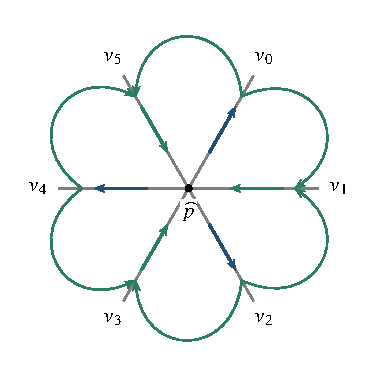
\includegraphics[width=.58\textwidth]{cd3-fig-02.pdf}
\FigureTag{CD3.2}{fig:cd3-02}
\end{figure}
As illustrated, we expect points on these rays to map into one another as indicated by the arrows. The orbit must eventually enter one of the domains
\[
\Delta_j=\{re^{i\theta}v_j:r>0,\ |\theta|<\pi/n\}
\]
and it must also approach $0$ asymptotically in an attracting direction $v_j$. We obtain the necessary bounds by conjugating the iterates to another hyperbolic surface and applying Pick's theorem. Define the biholomorphism
\[
\varphi\colon\Delta_j\longrightarrow\mathbb C\setminus\mathbb R_{(-1)^j},
\qquad\varphi(z)=\frac c{z^n},\quad c=-\frac1{na}.
\]
% Source page 4
On $\Delta_j$, $f(z)=z(1+az^n+o(z^n))$. Shift this to the slit plane $\mathbb C\setminus\mathbb R_{(-1)^j}$, and let $\psi_j=\varphi^{-1}$. Then
\[
f\circ\psi_j(w)=\sqrt[n]{\frac c w}\left(1+\frac{ac}{w}+o(1/w)\right),
\qquad w\in\mathbb C\setminus\mathbb R_{(-1)^j},
\]
where the $n$th root makes sense. Consequently,
\begin{align*}
F_j(w)=\varphi\circ f\circ\psi_j(w)
&=w\left(1+\frac{ac}{w}+o(1/w)\right)^{-n}\\
&=w\left(1-\frac{nac}{w}+o(1/w)\right)
=w\left(1+\frac1w+o(1/w)\right)\\
&=w+1+o(1).
\end{align*}
Writing the same calculation with big-$O$ notation yields
\[
F_j(w)=w+1+O\!\left(\frac1{\sqrt[n]{|w|}}\right).
\tag{*}\label{cd3:translation-estimate}
\]
This follows by writing $f(z)=z(1+az^n+O(z^{n+1}))$ and following the same steps. This estimate will be used below.
% Source page 5
For $|w|>R$, with $R$ large, $|F_j(w)-w-1|<1/2$. Thus $\Re F_j(w)>\Re w+1/2$.
\begin{figure}[H]\centering
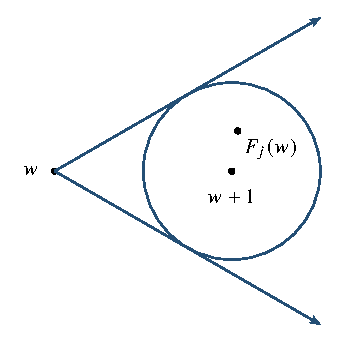
\includegraphics[width=.47\textwidth]{cd3-fig-03.pdf}
\FigureTag{CD3.3}{fig:cd3-03}
\end{figure}
When $|w|$ is large, $|\psi_j(w)|$ is small. Thus for small $|z|$,
$\Re\varphi(f(z))>\Re\varphi(z)+1/2$.
For the orbit $\{z_k\}_k$, this gives $\Re\varphi(z_{k+1})>\Re\varphi(z_k)+1/2$. Eventually $\varphi(z_k)\in\mathbb H_R$ for large $R$, and $F_j(\mathbb H_R)\subseteq\mathbb H_R$. Hence $f(\psi_j(\mathbb H_R))\subseteq\psi_j(\mathbb H_R)$. Call $\psi_j(\mathbb H_R)=P_j(R)$. Thus eventually all $z_k$ belong to $\Delta_j$ for some $j$.

Since $F_j(w)-w=1+o(1)$, putting $w_k=\varphi(z_k)$ gives $w_{k+1}-w_k\to1$, and
\[
\frac{w_k-w_0}{k}=\frac1k\sum_{h=0}^{k-1}(w_{h+1}-w_h)\longrightarrow1.
\]
% Source page 6
Thus $w_k/k\to1$, so $w_k\sim k$. Since $1/w_k=-naz_k^n$, we get $naz_k^n\sim-1/k$. As $nav_j^n=-1$, this gives $z_k^n\sim v_j^n/k$.

Write $z_k=r_ke^{i\alpha_k}$ and $v_j=re^{i\alpha}$. Then $z_k^n=r_k^ne^{ni\alpha_k}$ and $v_j^n/k=(r^n/k)e^{ni\alpha}$. The modulus of their ratio tends to one, so $r_k\sim r/k^{1/n}$. Also $e^{n(\alpha_k-\alpha)i}\to1$. Since eventually $z_k\in P_j(R)\subset\Delta_j$ and $|\alpha_k-\alpha|<\pi/n$, it follows that $\alpha_k-\alpha\to0$. Therefore $z_k\sim v_j/k^{1/n}$.
\end{proof}
Having seen this, let us identify the basin of attraction for $\widehat p$.
\setcounter{definition}{11}\begin{definition}
The set $\mathcal A_j(\widehat p)$ consists of all $p_0$ whose orbit $p_0\mapsto p_1\mapsto p_2\mapsto\cdots$ under $f$ tends to $\widehat p$ along $v_j$. Since $P_j(R)\subset\mathcal A_j(\widehat p)$, there is a unique connected component $\mathcal A_j^0$ with $f(\mathcal A_j^0)\subseteq\mathcal A_j^0$. This is called the immediate basin.
\end{definition}
% Source page 7
The construction above gives forward-invariant domains in $\Delta_j$ around $\widehat p$, but it does not yet show that their union surrounds $\widehat p$; gaps may remain. The domain $P_j(R)\subset\Delta_j$ satisfies $f(P_j(R))\subseteq P_j(R)$, and an orbit tending to $\widehat p$ along $v_j$ eventually enters it. Let us generalise this phenomenon.
\setcounter{definition}{12}\begin{definition}[Attracting and repelling petals]
Let $N$ be a neighbourhood of $\widehat p$ on which $f$ is univalent. A set $P\subset N$ is an attracting petal for $f$ at $\widehat p$, associated with an attracting vector $v_j$, if
\begin{itemize}
\item $f(P)\subseteq P$;
\item an orbit $\{z_k\}_k$ enters $P$ eventually if and only if $z_k\to\widehat p$ along $v_j$.
\end{itemize}
Repelling petals are defined similarly by considering $f^{-1}$ on $f(N)$.
\end{definition}
Clearly $P$ contains exactly one $v_j$; these sets therefore look like petals around the ``base branch'' $v_j$. The next theorem says that the attracting and repelling petals surround $\widehat p$: they fit together into a round flower.
% Source page 8
\setcounter{theorem}{17}\begin{theorem}[Flower theorem]\label{cd3:flower}
There are petals $\{P_j\}_{j=0}^{2n-1}$, each attracting or repelling, such that $\{\widehat p\}\cup P_0\cup\cdots\cup P_{2n-1}$ is an open neighbourhood of $\widehat p$. The sets $P_j$ and $P_j\cap P_{j\pm1}$ are simply connected regions, except when $n=1$.
\end{theorem}
\begin{proof}
We cannot simply take $P_j(R)$. The construction above gives the correct dynamics inside each sector, but these sets may leave gaps between adjacent attracting and repelling directions. We therefore modify $\mathbb H_R$ slightly. Let
\[
W_R=\{u+iv:u+|v|>2R\},\qquad\mathbb H_{2R}\subset W_R.
\]
For $R$ sufficiently large, the estimate $F_j(w)=w+1+o(1)$ gives
\[
F_j(W_R)\subset W_R,
\]
and the corresponding estimate for $F_j^{-1}(w)=w-1+o(1)$ gives
\[
F_j^{-1}(-W_R)\subset -W_R.
\]
Then
\[
P_j=\psi_j(W_R)\subset\Delta_j
\]
is an attracting petal for odd $j$, while
\[
P_j=\psi_j(-W_R)\subset\Delta_j
\]
is a repelling petal for even $j$.
\begin{figure}[H]\centering
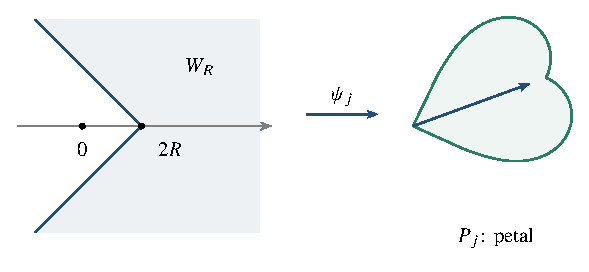
\includegraphics[width=.74\textwidth]{cd3-fig-04.pdf}
\FigureTag{CD3.4}{fig:cd3-04}
\end{figure}

Now note the following correspondence, since $\varphi$ preserves orientation because it is locally conformal away from $\widehat p$.
\begin{figure}[H]\centering
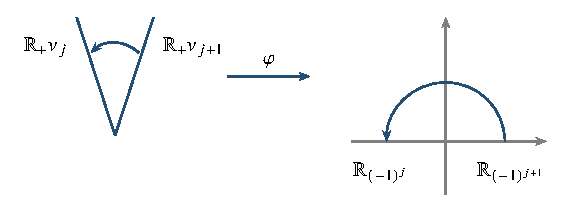
\includegraphics[width=.64\textwidth]{cd3-fig-05.pdf}
\FigureTag{CD3.5}{fig:cd3-05}
\end{figure}
Thus
\[
\varphi(\Delta_j\cap\Delta_{j+1})=
\begin{cases}
\text{upper half-plane},&2\mid j,\\
\text{lower half-plane},&2\nmid j.
\end{cases}
\]
The set $W_R\cap(-W_R)$ has exactly two simply connected components,
\[
V_R^+=\{u+iv:v>2R+|u|\},\qquad
V_R^-=\{u+iv:v<-2R-|u|\}.
\]
According to the parity of $j$, the map $\varphi$ carries $P_j\cap P_{j+1}$ onto $V_R^+$ or $V_R^-$. Hence $P_j$ and $P_j\cap P_{j\pm1}$ are simply connected, with the stated exception when $n=1$.

Finally, $W_R\cup(-W_R)$ contains $\{w:|w|>2R\}$. Since $\varphi(z)=c/z^n$, the union of the inverse images of these two sets contains a punctured disc about $\widehat p$. Therefore
\[
\{\widehat p\}\cup\bigcup_{j=0}^{2n-1}P_j
\]
contains a neighbourhood of $\widehat p$. This is the flower theorem, due to Leau and Fatou.
\begin{figure}[H]\centering
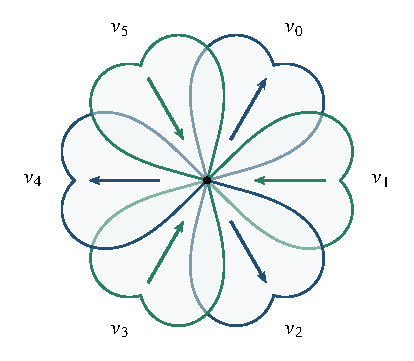
\includegraphics[width=.60\textwidth]{cd3-fig-06.pdf}
\FigureTag{CD3.6}{fig:cd3-06}
\end{figure}
\end{proof}
% Source page 10
We now ask the question suggested by the case $0<|\lambda|<1$: can we understand the dynamics separately on each of the $2n$ petals? The next theorem addresses this completely.
\setcounter{theorem}{18}\begin{theorem}[Parabolic linearisation]\label{cd3:linearisation}
For any petal $P$, there is a conformal embedding $\alpha\colon P\to\mathbb C$, unique up to translation, making the following diagram commute. In the literature, $\alpha$ is called a \emph{Fatou coordinate}.
\begin{figure}[H]\centering
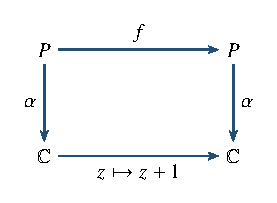
\includegraphics[width=.34\textwidth]{cd3-fig-07.pdf}
\FigureTag{CD3.7}{fig:cd3-07}
\end{figure}
\end{theorem}
\begin{proof}
We prove the assertion for an attracting petal; the repelling case follows by applying the same argument to $f^{-1}$. Recall that on $\mathbb H_R$,
\[
F_j(w)=w+1+O\!\left(|w|^{-1/n}\right).
\]
After increasing $R$, Cauchy's estimate on a slightly smaller region gives
\[
F_j'(w)=1+O\!\left(|w|^{-1-1/n}\right).
\]
Fix $\widehat w\in\mathbb H_R$ and set
\[
\beta_k(w)=F_j^{\circ k}(w)-F_j^{\circ k}(\widehat w).
\]
Since $\Re F_j^{\circ k}(w)>\Re w+k/2$, the mean-value integral along the segment joining $F_j^{\circ k}(\widehat w)$ to $F_j^{\circ k}(w)$ gives, locally uniformly in $w$,
\[
\left|\frac{\beta_{k+1}(w)}{\beta_k(w)}-1\right|
\le \frac{C}{k^{1+1/n}}
\]
whenever $w\ne\widehat w$ and $k$ is sufficiently large. The series $\sum_k k^{-1-1/n}$ converges, so the corresponding infinite product converges locally uniformly to a nonzero limit. Hence $\beta_k$ converges locally uniformly to a holomorphic map $\beta$.

The same estimate applied to any two distinct points $w,w'\in\mathbb H_R$ shows that
\[
\lim_{k\to\infty}\bigl(F_j^{\circ k}(w)-F_j^{\circ k}(w')\bigr)\ne0.
\]
Thus $\beta$ is univalent. Moreover,
\begin{align*}
\beta(F_j(w))
&=\lim_{k\to\infty}\bigl(F_j^{\circ(k+1)}(w)-F_j^{\circ k}(\widehat w)\bigr)\\
&=\beta(w)+\lim_{k\to\infty}
\bigl(F_j^{\circ(k+1)}(\widehat w)-F_j^{\circ k}(\widehat w)\bigr)\\
&=\beta(w)+1.
\end{align*}
The estimates also give $\beta(w)/w\to1$ as $|w|\to\infty$ within $\mathbb H_R$. If $U=\beta(\mathbb H_R)$, Rouch\'e's theorem applied on sufficiently large discs contained in $\mathbb H_R$ shows that
\[
\bigcup_{m\in\mathbb Z}(U+m)=\mathbb C.
\]

For $P=P_j(R)$, define
\[
\alpha(z)=\beta(\varphi(z)).
\]
For any $z$ in the full petal $P$, choose $k$ so that $f^{\circ k}(z)\in P_j(R)$ and define
\[
\alpha(z)=\alpha(f^{\circ k}(z))-k.
\]
This is independent of $k$, and it gives a conformal embedding satisfying
\[
\alpha(f(z))=\alpha(z)+1.
\]
\begin{figure}[H]\centering
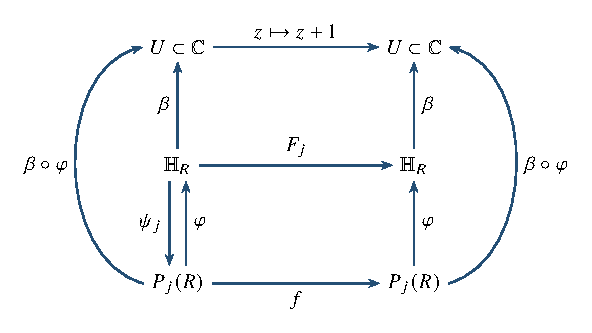
\includegraphics[width=.65\textwidth]{cd3-fig-08.pdf}
\FigureTag{CD3.8}{fig:cd3-08}
\end{figure}
\begin{figure}[H]\centering
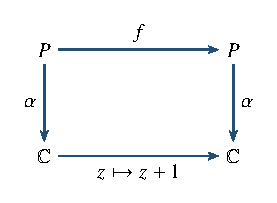
\includegraphics[width=.34\textwidth]{cd3-fig-09.pdf}
\FigureTag{CD3.9}{fig:cd3-09}
\end{figure}

For uniqueness, let $\alpha,\alpha'$ be two such Fatou coordinates, with images $U,U'$. Then $g=\alpha'\circ\alpha^{-1}$ satisfies $g(w+1)=g(w)+1$ whenever both sides are defined. Since the integer translates of $U$ cover $\mathbb C$, this relation extends $g$ to an injective entire map $\widehat g\colon\mathbb C\to\mathbb C$. Every injective entire map is affine, and the identity $\widehat g(w+1)=\widehat g(w)+1$ forces $\widehat g(w)=w+b$. Therefore $\alpha'=\alpha+b$.
\end{proof}
\begin{remark}
Critical points again play a crucial role; we will not elaborate on this. If $\alpha$ is the Fatou coordinate for the petal wrapping $v_j$, it extends to $\mathcal A_j(\widehat p)$, and $\alpha^{-1}$ extends to some $\mathbb H_R$ with $R$ optimal. This is analogous to the Koenigs-coordinate situation. For every $\mathcal A_j(\widehat p)$ there is a maximal petal $P_{\max}\subseteq\mathcal A_j(\widehat p)$ to which $\alpha$ extends biholomorphically, and $f$ has a critical point on $\partial P_{\max}$ that prevents further univalent extension.
\end{remark}
\begin{remark}
We have $\alpha(z)\to\infty$ as $z\to0$, and $0$ is a parabolic fixed point. The preimages $\{f^{-n}(0)\}$ form a dense subset of the basin boundary, obstructing expansion of $\alpha$.
\end{remark}
\begin{remark}
In conclusion, the $\mathcal A_j(\widehat p)$ are disjoint basins with $\partial\mathcal A_j(\widehat p)\subseteq J$. Each basin has a Fatou coordinate describing its local behaviour on a maximal petal $P_{\max}$.
\end{remark}
% BLOG-CONTENT-END
\end{document}
